\section{Terms, definitions and concepts}
This section defines the terms which are used by CloudMan. 

\subsection{Regions}
A region in CloudMan can be single computer center or a set of computer centers making up a single entity, for example a site. Regions are distinct and independent computer centers. 

\subsection{Resource types}
In the Aldebaran release, a resource type was used as a minimal unit in which resources could be allocated. This idea turned out to be little useful, and added an unexpectedly large amount of additional issues. 

For Betelgeuze, resource types are redefined. We distinguish two different types:
\begin{itemize}
\item allocatable resources
\item not allocatable resources, or features
\end{itemize}
As an example, CPU resources are allocatable while the fact that machines in a specific zone (see below for the definition) have a UPS is a feature which cannot be allocated, that is you cannot sum them up and give a share of it to somebody as you can do for CPU or disk resources. 

Resource types are defined through the web interface and stored in the database. Not allocatable resources types require the following information:
\begin{itemize}
\item A name which identifies the resource. This name is used on the CloudMan interface when displaying the resource and it's usage. 
\item A floating point number indicating the price of this feature. The more expensive the resource is the higher the number should be. The aim of this number is to help the administrator to define the possible cost of resources in zones which provide this feature or resource. It must be possible to edit this number for existing resources. 
\end{itemize}
Allocatable resources require {\bf in addition} to the above the following information:
\begin{itemize}
\item A value (in general a floating point value)
\item A unit (stored as a string). This unit determines the unit in which the value is stored in the database
\item A list of alternate units along with a conversion rule which relates the new unit to the original one stored in the database 
\end{itemize}

As an example, {\it CPU resources} are measured in {\it HS06} which is a floating point number but can also be given in {\it kSi2k}. 
The actual value is filled in at the zone level, see below.

\subsection{Zones}
A zone is a specific part of a {\it region}. Each region is made up of one or more zones. As an example, a zone can map to a hardware installations with specific features, like batch nodes or machines for storage. 

A zone is defined by the allocatable and non allocatable resource which it provides. 
When a new zone is created, the administrator describes it by the different resources which it provides. For allocatable resources he needs to define the actual value of the resource (or amount of this resource) which is provided by this zone. 

A measure for the cost is defined for each zone as a floating point number. 
It is set manually when the zone is allocated, depending on its features and resources. The field must be editable, the unit is arbitrary. The higher the number, the higher the cost of resources in this zone.

{\bf Note:} Care must be taken in how zones in CloudMan are defined. Example: Let's assume that a site has two distinct computer centers. These computer centers are physically distinct, but the site runs a batch farm which spans over the two computer centers transparently to the users. In this case, all computing resources seen by the batch farm for public use should belong to the same zone in the CloudMan sense. Else, top level allocations could set additional quotas which may result in a fragmentation of resources. 

The relationship of regions and zones for a case like  CERN with several computer centers is shown in fig.~\ref{cerncase}.
\begin{figure}
\begin{center}
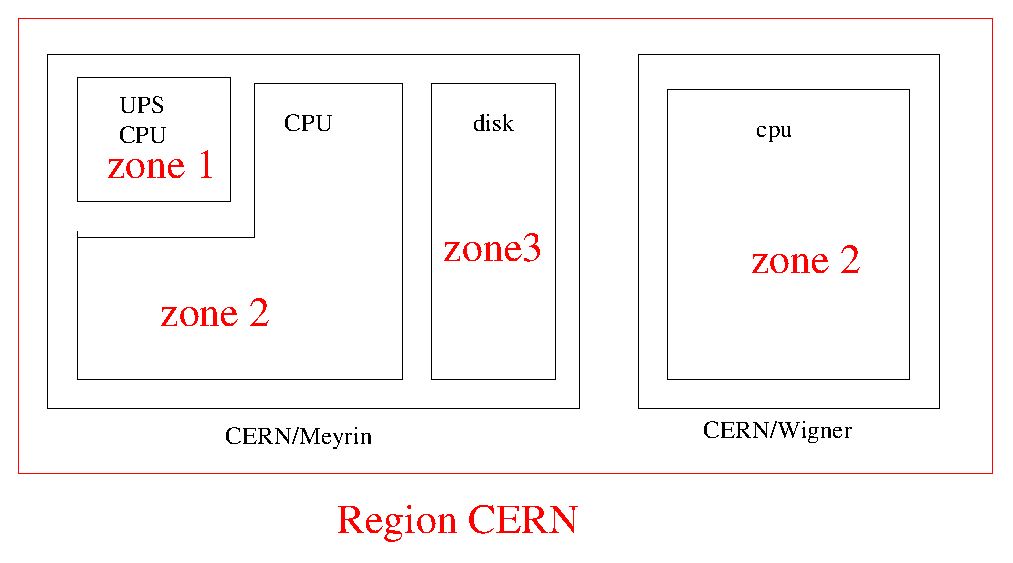
\includegraphics[width=\textwidth]{cerncase.eps}
\caption{\label{cerncase}Simplified scenario for CERN. It is assumed that there are two distinct computer centers which look like one large site. As an example the batch resources spread over the two computer centers. Therefore, only one region is present. Within this region there are CPU resources under UPS coverage, cheap CPU resources and disk resources. Similar resources which spread over the different computer centers still belong to the same zone.}
\end{center}
\end{figure}

\subsection{Groups}
In the previous release of CloudMan there was the concept of groups. For the CERN deployment, groups are handled by e-groups, therefore the CloudMan groups were nothing but a pointer to e-groups. As of Betelgeuze this concept is dropped and replaced by directly giving the e-groups name.

\subsection{Top level allocations}
In the CloudMan configuration files, it is possible to define a group of CloudMan administrators. These people are the only once who are allowed to perform top level allocations. A top level allocation is the assignement of a specific quantity of a resource to a user group. Top level allocations are done per zone and region. This way top level allocations set quotas on the possible usage of specific zones. 
\begin{table}[htb]
\begin{center}
\begin{tabular}{|l|l|l|l|}
\hline
Zone & total & experiment name & allocation \\
\hline
Nr. 1, UPS covered & 10 servers, 100HS06 each & CMS &  100 HS06 \\
Nr. 2, simple CPU  & 100 servers, 100HS06 each & CMS & 900 HS06 \\
\hline
\end{tabular}
\end{center}
\caption{\label{toplevelCMS}Example top level allocation for CMS: There are two zones, one with UPS coverage which has 10 servers, and one with 100 servers for CPU processing. The performance of each server corresponds to 100~HS06. CMS gets a total allocation of 1000~HS06, 10\% of which are UPS covered.  Cost of resources in zone 1 are larger than those in zone 2 due to the UPS feature.}
\end{table}
An example top level allocation is shown in table~\ref{toplevelCMS}.

\subsection{Projects}
A project is a service which is provided by the computer center and to which users can subscribe, in case they have got a top level allocation which is required for this service. Only CloudMan admins can create projects.  As an example, a computer center can offer computing resources in a batch farm so the CloudMan administrator would allocate a project {\it batch} to which all user groups who got a top level computing resource allocation can sign up. 

Table~\ref{projects} gives an example of project 
\begin{table}[htb]
\begin{center}
\begin{tabular}{|l|l|l|l|}
\hline
Project name & requirements & attributes & limitations\\
\hline
public batch & CPU resources & SHARE & maximum recursion depth 2 \\
vobox & CPU resources, UPS coverage & none & none \\
IaaS self service & CPU resources & none & none \\
\hline
\end{tabular}
\end{center}
\caption{\label{projects}Example projects which are allocated by the CloudMan administrator. There are 3 only here: public batch is owned by some group in IT which manages the batch farm. The idea of this project is to setup shares for large user groups. The vobox project is a service where experiments can get reliable resources which are covered with a UPS. This project will only use resource from Zone 1 in fig~\ref{cerncase} while the batch project will use only resources from Zone 2 because they are cheaper. The attribute SHARE indicates that these are shared (not dedicated) resources. The maximum recursion depth means that for this project it is possible to do group and subgroup allocations only, and not beyond that. The IaaS self service is meant for cheap development machines. It uses the same resources as the public batch project.}
\end{table}

\subsubsection{Project requirements}
In general, different projects will come with different service level agreements (SLA). In order to be able to fulfill these SLAs some projects will require specific features for the resources to be allocated to them, and thus enable only specific zones. 
When selecting resources , the cheapest matching option should be chosen to allocate resources. 
As an example, a site may run a batch farm and a service for critical applications. There will be two projects: a batch project with a requirement to select CPU resources, and a VOBOX\footnote{This is a CERN specific term for a service to give resources for critical applications to user communities/experiments} service which will require UPS coverage. 

\subsubsection{Project attributes}
When creating a project it must be possible to define attributes. An attribute is a key-value pair which is required to configure the project. At the project level it must be possible to provide a default value which is used if the user does not provide a value when assigning resources to this project. 

Project attributes are exported as key-value pairs so that they are available to the backend which configures the project. 

\subsubsection{Recursion limitation}
A special project attribute is a limitation on the recursion deps. By default there is no limitation on the maximum depth on group and subgroup allocations. In order to keep the complexity of some of the backends limited it may be necessary to restrict such allocations down to the subgroup level, for example. 


\begin{table}[htb]
\begin{center}
\begin{tabular}{|l|l|l|}
\hline
Project name & Administrator & Allocation \\
\hline
public batch & CMS\_batchadmin& 80\%\\
vobox & CMS\_VOC & 10\%\\
IaaS self service & CMS\_all& 10\% \\ 
\hline
\end{tabular}
\end{center}
\caption{\label{projectsAllocation} Project allocation for the example CMS group. These allocations are done by the CMS administrator who can sign up to any project for which he has a matching resource allocation. For each project he's interested in he determines a responsible (group of people), and gives them a fraction of the resources he got from the CloudMan administrator. With 10\% of the total allocation in the UPS they fill up their quota there.}
\end{table}

\subsection{Project allocations}
A project allocation is an assignement of resource to a specific project. This can be done by any member of a group which got a top level allocation for a resource which is required by the project. A project allocation is taken from a top level allocation for a specific project. When doing a project allocation a group of people the project allocation managers  have to be specified who will manage this project allocation in the future.

Table~\ref{projectsAllocation} gives an example of how a project allocation works. 

\subsection{Group and sub-group allocations}
Project allocation managers got an allocation of resources for a specific project. These people can delegate further management of these resources to another group of people who in turn can reallocate their bit of the cake to other people (sub-group allocations). 
The maximum depth of group, subgroup, sub-subgroup etc allocations is a feature which is project specific. It must be possible to restrict the recursion depth per project. This is illustrated in table~\ref{groupAllocationForBatch} and ~\ref{subgroupAllocationForBatch} for the batch project in our example.

\begin{table}[htb]
\begin{center}
\begin{tabular}{|l|l|l|}
\hline
Group name & Administrator & Allocation \\
\hline
HiggsSearchers & CMSHiggsAdmins& 80\%\\
Other & CMS\_batchadmin & 20\%\\
\hline
\end{tabular}
\end{center}
\caption{\label{groupAllocationForBatch}Group allocations for the batch project as done by the CMS\_batchadmin. The Higgs search group gets a large share of the batch system share of CMS. They can further on set priorities by defining shares for the individual Higgs search teams.  }

\end{table}

\begin{table}
\begin{center}
\begin{tabular}{|l|l|l|}
\hline
SubGroup name & Administrator & Allocation \\
\hline
HiggsChannelA & CMSHiggsAdmins& 25\%\\
HiggsChannelB & CMSHiggsAdmins& 25\%\\
HiggsChannelC & CMSHiggsAdmins& 25\%\\
HiggsChannelD & CMSHiggsAdmins& 25\%\\
\hline
\end{tabular}
\end{center}
\caption{\label{subgroupAllocationForBatch}Group allocations for the batch project as done by the CMS\_batchadmin. The Higgs search group gets a large share of the batch system share of CMS. They can further on set priorities by defining shares for the individual Higgs search teams. Due to the limitation in the recursion depth in the batch project it is not possible for the CMSHiggsAdmins to further split up the resources. }
\end{table}

\subsubsection{Group and subgroup attributes}
Group and subgroup allocations belong to a specific project. When doing such an allocation, it must be possible to update the values of the attributes which are required by the project. If no new value is given, it is inherited from the hierarchy above.  


\section{Buisiness continuity}
If a site has two distinct computer centers it may want to distribute all services in a way which allows it to continue to work even if one of the two centers goes down. Services and applications have to be able to support such a scenario. From the infrastructure point of view it requires that all relevant services to have one leg in each of the computer centers. 
In a fully virtualized computer center this requirement is one on the scheduling policies: instead of filling up hypervisors one by one VMs belonging to the same project have to be distributed over the two centers. 

In Cloudman this can be done if all zones for the relevant services spread over the two computer centers. Projects supporting this option should have a flag which indicates that the resources should be distributed over the two centers rather than being filled up one by one. The flag is implemented as a special project attribute. This will be visible from the low level export layer to the backend which configures the project. 



